\section{Étude des solutions d'architecture}

Dans cette partie nous allons vous présenter deux scénarios décrivant des directives à prendre pour l'entreprise. Pour se faire, nous avons étudié avec précision l'existant de l'entreprise. Nous nous sommes donc appuyé sur les données de l'entreprise pour définir ces scénarios. \\
Nous présenterons dans un premier temps le scénario d'urbanisation du S.I. puis dans un deuxième temps le scénario de déploiement d'un E.R.P.

\subsection{Scénario d'urbanisation du S.I.}

Afin de répondre aux besoins exprimés par le client, nous proposons une première solution de déploiement basée sur une architecture d'intégration d'application, autrement dit E.A.I. 
En effet, l'un des principaux constats effectués après l'analyse de l'existant de l'entreprise est que cette dernière possède bien un S.I. performant et adapté à ses besoins, du moins dans la partie opérationnelle. En ce qui concerne le coté analytique cela se révèle un peu moins proche de la réalité, ceci est notamment lié à la vétusté des équipements en activité.\\ 
L'objectif principal du scénario proposé est de tirer parti de cet existant, en le restructurant et en le rendant évolutif afin de se conformer à vos exigences.

\subsubsection{Lignes directrices du projet}

Nous avons donc décidé de proposer une architecture typée par site. Plusieurs clés pour cette architecture :\\

\begin{itemize}
\item Réplication des services par site, permettant un fonctionnement assuré en mode dégradé du S.I.
\item Typage du S.I. des différents sites relativement aux services utilisés sur ces derniers
\item Intégration des applications opérationnelles existantes dans d'une architecture typée E.A.I.
\item Déploiement d'une orchestration de service S.O.A.
\item Refonte du segment datawarehouse et business intelligence, avec des problématiques de qualité\\
\end{itemize}

Afin d'optimiser le fonctionnement de votre entreprise, nous prévoyons d'intégrer un système d'orchestration de services S.O.A., basé sur la modélisation de vos activités sous forme de processus industriels, formant votre chaîne de valeur.\\
Chaque entité de l'entreprise possède sa propre base de données opérationnelle, servant d'entrepôt de données local à chaque site. Chaque application opérationnelle déployée est synchronisée par un connecteur E.S.B. développé spécifiquement, ainsi chaque site possède son propre sous ensemble de datawarehouse, qui est ensuite synchronisé et intégré au datawarehouse principal, hébergé à la D.S.I. du site central. Ainsi, si le WAN de l'entreprise est indisponible, le mode de fonctionnement dégradé permet d'éviter l'arrêt de vos activités.\\
Notons aussi, le déploiement d'un système de Master Data Management pour la qualité globale des données hébergées. Ce système à la pointe de la technologie des systèmes d'information permet d'assurer une gestion de la qualité du premier ordre dans votre système d'information.\\
Enfin, nous prévoyons une refonte complète de la partie analytique de votre entreprise, afin d'y intégrer une suite analytique de dernière génération pour le suivi de vos activités, et des outils de fouille de données pour effectuer de l'analyse prédictive.\\

Ainsi, comme nous allons le découvrir, cette architecture permettant de mettre à profit un existant déjà performant et adapté à vos besoins, permet d'envisager à nouveau un système évolutif, doté des dernières technologies en terme de qualité de données et de business intelligence, permettant un pilotage de vos activités le plus précis possible.\\

\subsubsection{Architecture \& Services hébergés}

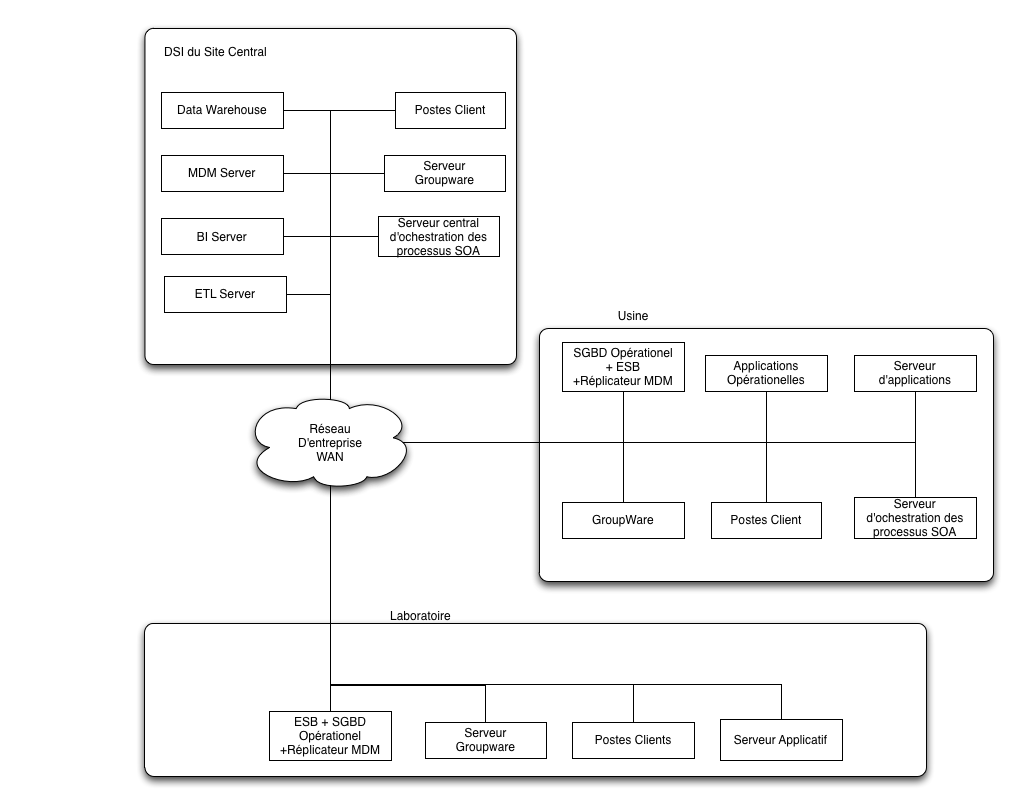
\includegraphics[scale=0.2]{DiagrameSOAPdc4.png}

\subsubsection{Infrastructure de support technique}
Afin de simplifier l'exploitation, nous proposons que l'architecture logicielle proposée soit supportée par une architecture basée sur des machines virtuelles, limitant grandement le nombre de machines de type serveur à déployer.
Les systèmes virtuels sont facilement manipulables et peuvent être restaurés simplement en cas de défaut de machines. Ce qui simplifie grandement les tâches d'administration.\\
Bien entendu les infrastructures de transport, passives et actives sont à prévoir sur les différents sites, si elles n'existent pas déjà.

\subsubsection{Architecture pour le site central}

Le site central est dans ce scénario le centre névralgique du système d'information de l'entreprise. Les services hébergés sont les suivants :\\

\begin{itemize}
\item Main datawarehouse : Principal entrepôt de données de l'entreprise, c'est lui qui constitue la base de travail pour les applications de business intelligence.
\item M.D.M. Server : Serveur de Master data Management, en charge de la génération, du maintien, et de l'exposition aux applications utilisatrices de la base d'exploitation de données de références.
\item B.I. Server : Hébergement des principaux services de business intelligence, système de génération de rapports, générateurs de tableaux de bords et applicatif dédié au DataMining.
\item E.T.L. Server : En charge de l'alimentation du datawarehouse, assure la synchronisation des données entre les différents S.G.B.D. opérationnels déployés sur les différents sites, et la synchronisation réciproque entre le datawarehouse et le système de master data management.
\item Serveur central d'orchestration S.O.A. : Serveur en charge de l'orchestration des principaux processus et méta-processus de l'entreprise, il pilote les services d'orchestration déployés dans chaque site.
\item Serveur Groupware, dédié au travail collaboratif.
\end{itemize}

La totalité des postes présents sont réutilisés, moyennant éventuellement un redéploiement de ces derniers. De plus, la création d'une D.S.I. implique l'équipement des effectifs de ce service.

\subsubsection{Architecture pour laboratoire \& Usine}

Chaque entité de l'entreprise possède son propre S.I. autonome, permettant un fonctionnement de l'entreprise en mode dégradé (site principal in-joignable, etc...).
Toute la finesse de la solution se trouve au niveau de la décentralisation des bases de données opérationnelles, qui sont par la suite agrégées au niveau du site principal \\
Pour parvenir  à cela, nous dotons le serveur de base de données de trois fonctionnalités principales.
\begin{itemize}
\item S.G.B.D. : Serveur de base de données classique, hébergeant toutes les données opérationnelles nécessaires au fonctionnement du site.
\item E.S.B. : Système de synchronisation et de communication entre le serveur de base de données et les application opérationnelles utilisatrices.
\item M.D.M. réplication Server : Serveur de rapatriement et de stockage des données de références du S.I., permettant l'exploitation des données de références nécessaire au fonctionnement des application opérationnelles.
\end{itemize}

Ensuite, les services proposés sont bien évidemment adaptés aux besoins des différents sites. Notons tout de même la présence d'un serveur d'orchestration S.O.A. déporté pour contrôler les processus de fonctionnement des sites, très utile pour les usines de fabrication notamment, où l'avantage d'avoir une maîtrise de l'activité par processus n'est plus à démontrer.

\subsubsection{Nouveaux services envisagés}

L'architecture proposée possède donc l'avantage avant tout de mettre en place une infrastructure évolutive, ou le développement et l'intégration de nouveaux services opérationnels destinés à couvrir vos objectifs pour le système d'information.

\begin{itemize}
\item S.S.O. / LDAP / CAS : Nous prévoyons la mise en place d'un système de centralisation des identités dans le S.I., afin d'en augmenter la sécurité et l'extensibilité, notamment via l'intégration aux fournisseurs.
\end{itemize}

\subsubsection{Robustesse et tolérance aux incidents}

Compte tenu de l'architecture détaillée auparavant, nous avons réussi à limiter sur de nombreux aspects les risques pour le système d'information.\\

\subsubsection* {Mode dégradé}

Du fait de son architecture hautement décentralisée et des mécanismes de synchronisation issues des dernières technologies en date, le système d'information de chaque site reste opérationnel même si la liaison entre le site central et les sites distant n'est plus opérationnel. De plus, la cohérence des données n'est en aucun cas remise en question les outils d'E.A.I., E.S.B. et autres Data Management sont là pour assurer le tout !

\subsubsection*{Réplication Géographique}
Autre point positif, les données sont automatiquement répliquées entre les différents sites et le site central, chaque site pouvant avoir besoin des données opérationnelles d'un autre site.\\
Ainsi, en cas de sinistre important sur l'un des sites, les risques de perte de données seront minimisés car ces dernières sont automatiquement répliquées sur les autres sites et le serveur central.

\subsubsection{Impact organisationnel}

Deux points de vue en réponse à cette question\\
\begin{enumerate}
\item Internalisation des compétences : création d'une D.S.I., et embauche des personnels ayant la compétence de développement des connecteurs d'intégration, de déploiement et de maintenance de l'installation par étape. Ce choix ayant un coût fixe, il permet d'éviter de créer un lien de dépendance entre vous et une entreprise prestataire de services en informatique.
\item Externalisation de la maintenance informatique : il s'agit d'évaluer et de vérifier que votre actuel prestataire possède les compétences nécessaires pour effectuer ce type de démarche, qu'il s'avère relativement difficile d'externaliser au final, du fait de la phase de développement spécifique, nécessitant un temps relativement long entre la première recette et la phase de stabilité opérationnelle.
\end{enumerate}

\subsubsection{Quelques chiffres clés du scénario}
\begin{figure}[H]
\begin{center}
 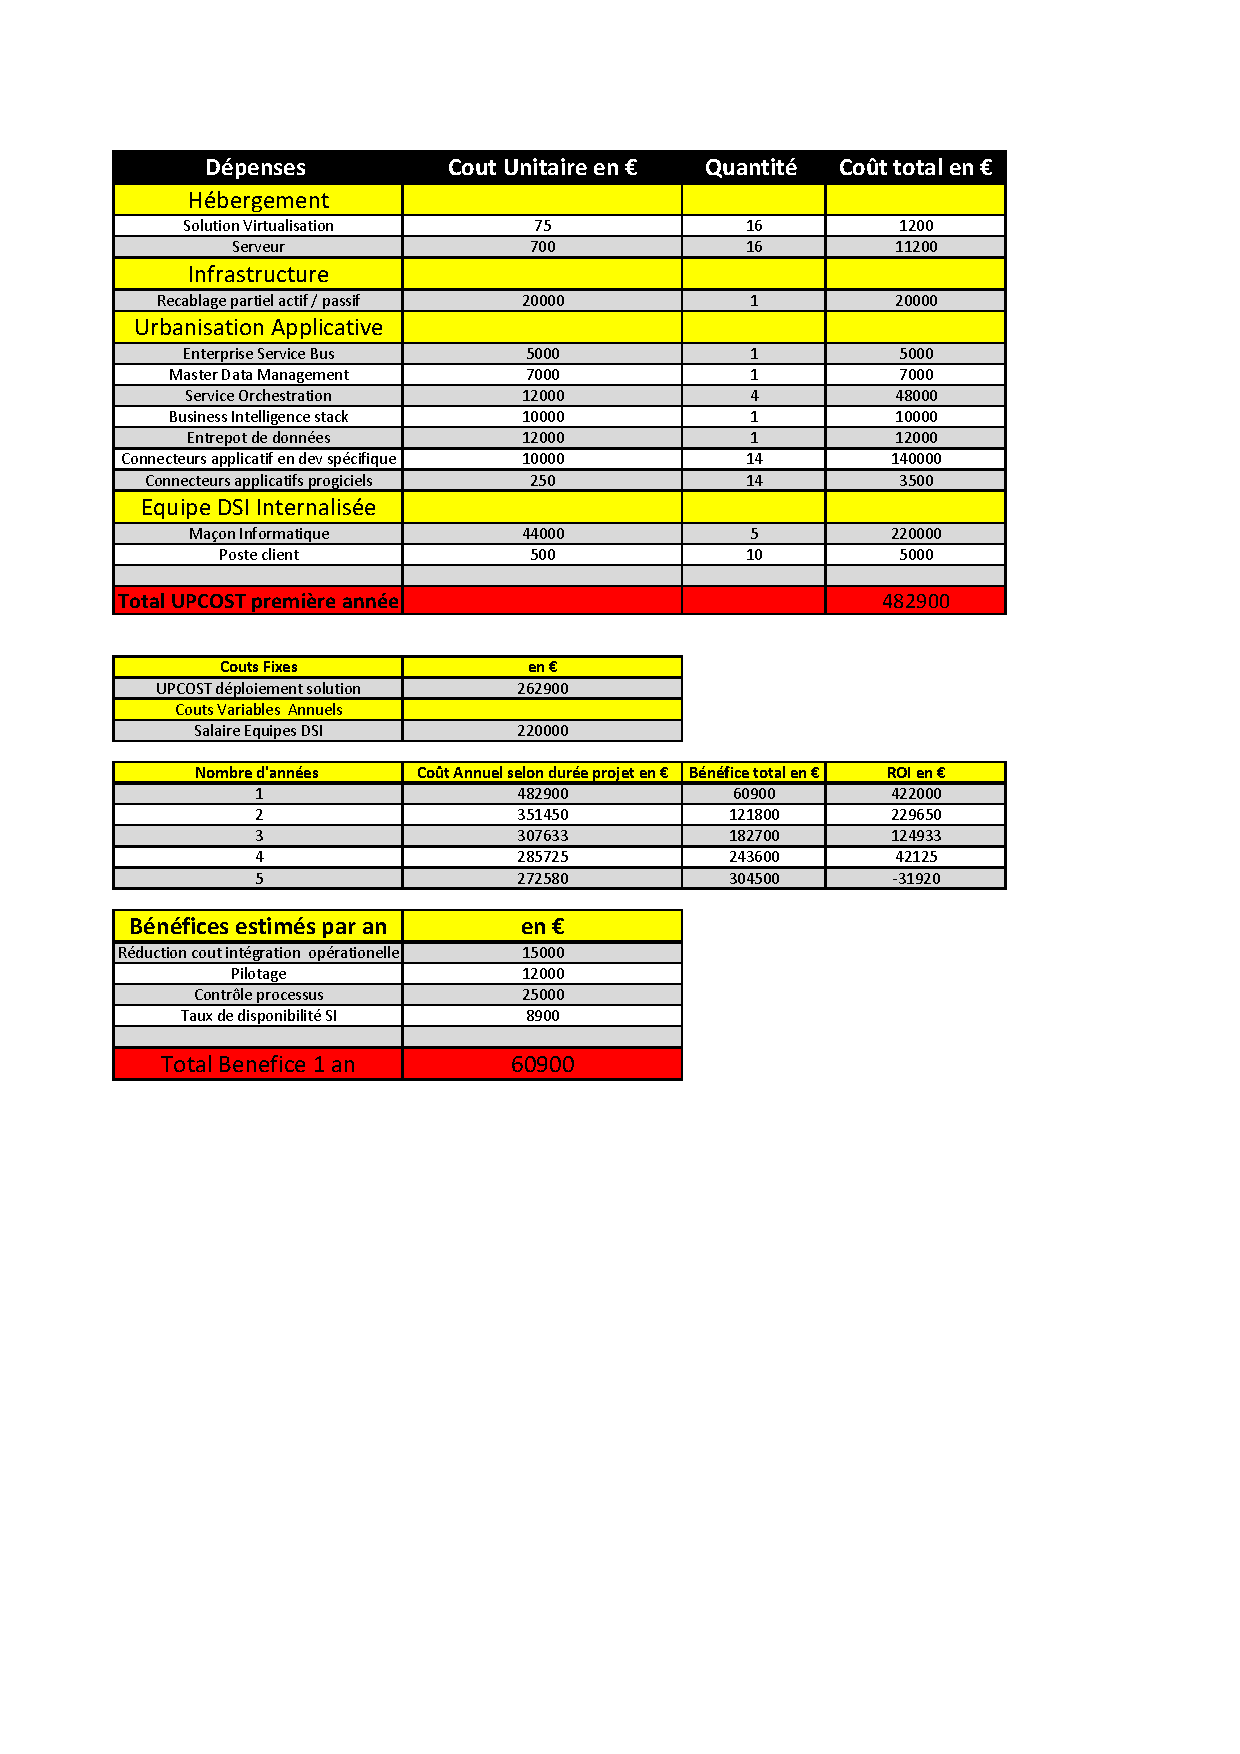
\includegraphics [scale=0.5]{ChiffresScenario1.pdf}
\end{center}  
\end{figure}

\newpage
\subsection{Scénario de déploiement d'un ERP}
Nous avons pu constater qu'actuellement le S.I. de l'entreprise fonctionnement parfaitement bien. Nous proposons donc un scénario qui s'intègre au S.I. \\
Le scénario que nous allons décrire ci-dessous est une directive à prendre pour l'entreprise pour les 5 années à venir. Nous proposons à l'entreprise d'intégrer un E.R.P. et plus particulièrement des modules adaptés à ses différents objectifs de perfectionnement.  
\subsubsection{Présentation de la solution}
Cette solution consiste à intégrer au système existant un système d'E.R.P. pour répondre aux besoins B2B de l'entreprise. Il propose des applications spécialisées pour la gestion des laboratoires (LIMS), de la relation client (C.R.M.), de la maintenance (G.M.A.O.). Actuellement l'entreprise possède un S.I. fonctionnel et performant c'est pourquoi il n'est pas nécessaire de le modifier. Cependant, il est intéressant pour l'entreprise de rajouter des fonctionnalités de gestion de certain processus. L'entreprise est composée d'un laboratoire central, structure contenant des données confidentielles ; pour le moment sa gestion est similaire aux autres structures : usines, sièges et service central de maintenance. La solution que nous présentons dans ce scénario s'adapte parfaitement à l'entreprise en proposant un module dédié à la gestion du laboratoire, mais également aux autres besoins de l'entreprise : outils de pilotage, processus dédiés au B2B.   
\paragraph{Architecture Applicative}
Voici une représentation des domaines qui seront gérés par le scénario que nous proposons de mettre en place :
\begin{figure}[H]
\begin{center}
 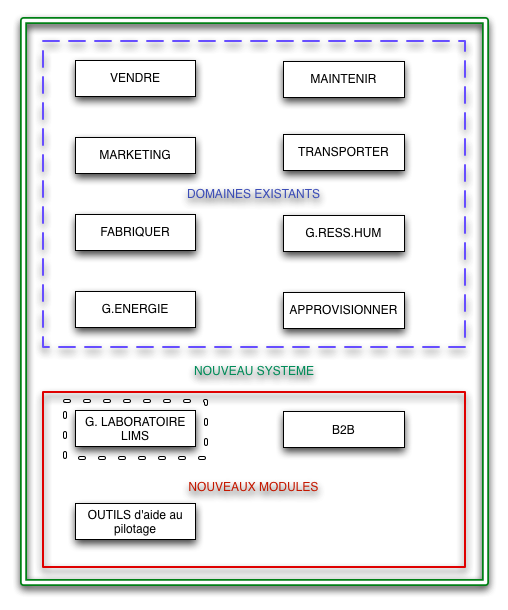
\includegraphics[scale=0.5]{ERPsolution.png}
  \caption{Nouveau système}
\end{center}  
\end{figure}

Nous proposons d'intégrer aux domaines existants : vendre, marketing, approvisionner, etc.  des modules supplémentaires permettant d'une part la gestion du laboratoire, d'autre part le déploiement d'outils d'aide au pilotage et pour finir des processus permettant la gestion du B2B.\\
Le module dédié à la gestion du laboratoire sera spécifique est développé pour correspondre au mieux à l'entreprise. En ce qui concerne les modules de B2B et les outils d'aide au pilotage nous proposons d'utiliser ceux existants. Nous savons qu'actuellement les grandes entreprises d'E.R.P. propose des modules configurables.   
\paragraph{Architecture Logicielle}
Cette solution ne nécessite pas de logiciel mais d'héberger un soft sur un serveur. Chaque poste aura accès au système via un site internet. Il n'y a donc pas d'installation particulière à faire au niveau des sites.
\paragraph{Architecture matérielle}
Pour pouvoir mettre en place cette solution, nous allons devoir installer au niveau d'EDS un serveur dédié à la base de données. Chaque site aura donc accès à une base de données en locale qui sera mise à jour une fois par jour : la nuit. Cette architecture permet à chaque site d'avoir un accès rapide à la base de données. Les données des laboratoires seront transférées vers un serveur sécurisé. 
\subsubsection{Ressources nécessaires}
Pour le déploiement d'une telle solution, on peut envisager deux cas : soit on embauche du personnel dédié à l'intégration d'E.R.P. soit on sous-traite via une société spécialisée dans le domaine.
\subsubsection{Gestion du changement}
Pour permettre aux utilisateurs d'avoir une transition facile nous vous proposons un plan de déploiement comprenant des formations dédiés aux personnels concernés et un accompagnement vers le changement.
\subsubsection{Bilan financier}
Vous trouverez plus bas une représentation graphique résumant les principaux coûts de la solution, une étude approfondie sera bien évidemment nécessaire pour avoir un budget détaillé. Cependant ces premiers chiffres nous permettent d'avoir une estimation du montant final de la solution.
\begin{figure}[H]
\begin{center}
 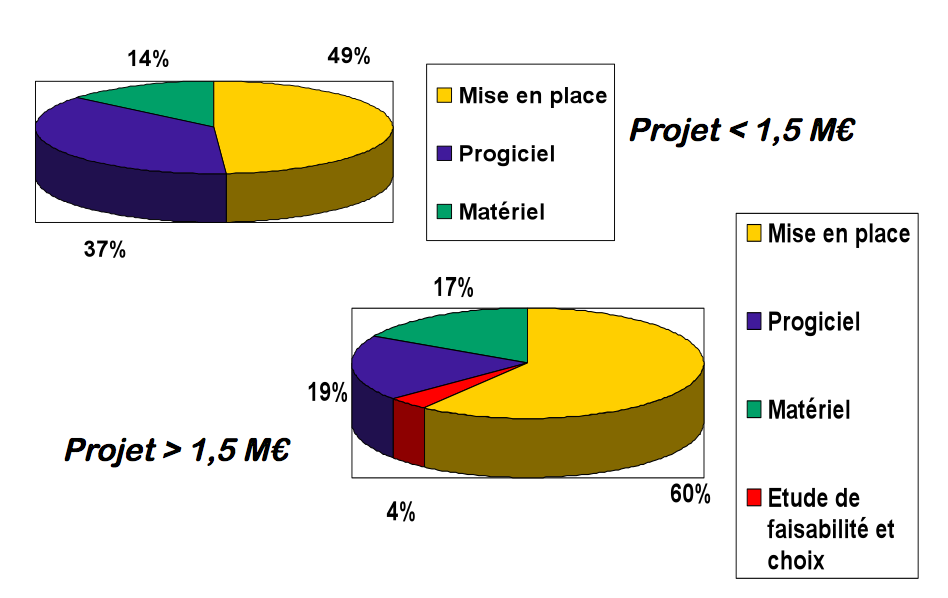
\includegraphics[scale=0.4]{CoutSolution.png}
  \caption{Analyse du cout du scénario}
\end{center}  
\end{figure}
\subsubsection*{Chiffrage détaillée}
\begin{figure}[H]
\begin{center}
 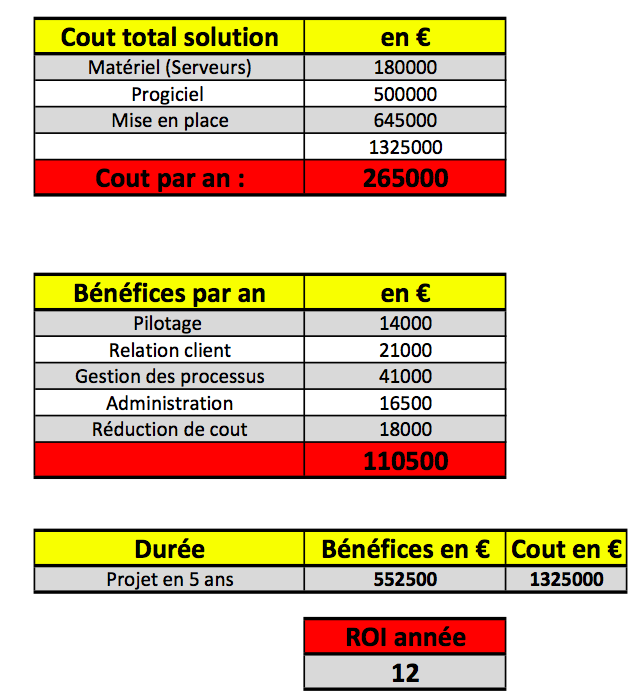
\includegraphics[scale=0.5]{ChiffresScenario2.png}
\end{center}  
\end{figure}


\subsubsection{Points forts, points faibles de la solution}
Cette solution répond pleinement aux besoins de l'entreprise concernant l'augmentation de sa réactivité vis à vis des fournisseurs et l'augmentation de ses services auprès de ses clients. Elle permet également d'améliorer le pilotage de l'entreprise grâce au module dédié à cette fonction.\\
La mise en place d'un E.R.P. est de plus en plus fréquent au sein des entreprises, c'est un système fiable qui permet : 
\begin{itemize}
\item[.]l'optimisation des processus de gestion;
\item[.]la cohérence et l'homogénéité des informations (un seul fichier article, un seul fichier client, etc.) ;
\item[.]l'intégrité et l'unicité du Système d'information ;
\item[.]le partage du même système d’information facilitant la communication interne et externe ;
\item[.]la minimisation des coûts : pas d’interface entre les modules, synchronisation des traitements, maintenance corrective simplifiée car assurée directement par l'éditeur et non plus par le service informatique de l'entreprise (celui-ci garde néanmoins sous sa responsabilité la maintenance évolutive : amélioration des fonctionnalités, évolution des règles de gestion, etc.) ;
\item[.]la globalisation de la formation (même logique, même ergonomie) ;
\item[.]la diminution du nombre de salariés ayant pour mission principale la saisie comptable (aide-comptable);
\item[.]la maîtrise des coûts, des délais de mise en œuvre, de déploiement ;\\
\end{itemize}

Il faut tout de même savoir que la solution proposée présente certains risques : 

\begin{itemize}
\item[•]la mise en œuvre peut être complexe si le périmètre est mal déterminé ou trop mouvant ou le projet mal piloté ;
\item[•]un coût élevé de 300 000 € minimum pour un progiciel fiable et de qualité, mais pouvant rapidement monter beaucoup plus haut, en fonction de l'industrie et de la complexité du projet. L'option fonctionnellement riche des solutions de logiciels libres si elle réduit les coûts de licence, ne supprime pas les coûts d'accompagnement et de formation ;
\item[•]le périmètre fonctionnel souvent plus large que les besoins de l'organisation ou de l'entreprise (le progiciel est parfois sous-utilisé) ;
\item[•]la nécessité d'une maintenance continue ;
\item[•]la captivité vis-à-vis de l'éditeur : le choix d'une solution est souvent structurant pour l'entreprise 
\item[•]le changement de P.G.I. peut être extrêmement lourd à gérer.
\end{itemize}

\subsection{Conclusion}
Cette partie aura permis de mettre en lumière deux directives que l'entreprise peut être amenée à suivre pour répondre à ses objectifs définis dans son schéma directeur. La liste des scénarios est exhaustive, nous avons décris les deux scénarios qui nous paraissait les plus pertinents.   